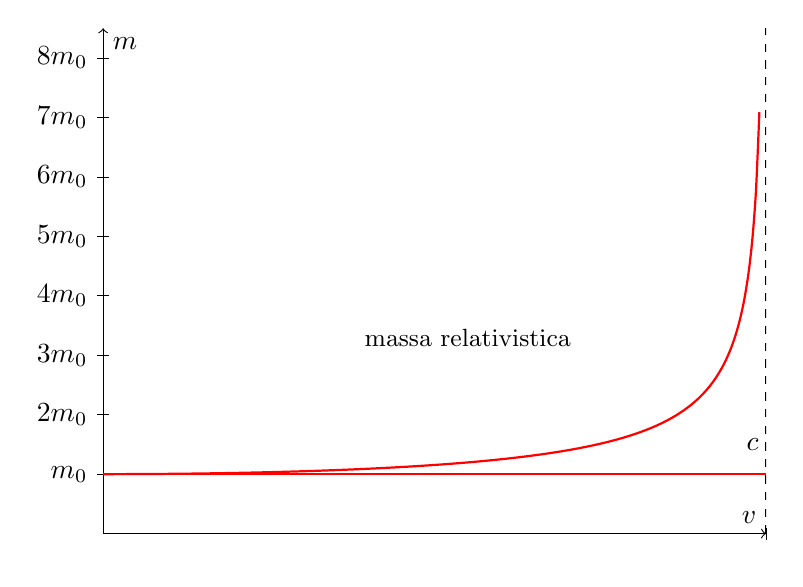
\begin{tikzpicture}

\begin{axis}[
    axis lines=middle,
    xlabel={$v$},
    ylabel={$m$},
    xmin=0, xmax=1,
    ymin=0, ymax=8.5,
    xtick={1},
    xticklabels={},
    ytick={1,2,3,4,5,6,7,8},
    yticklabels={$m_0$, $2m_0$, $3m_0$, $4m_0$, $5m_0$, $6m_0$, $7m_0$, $8m_0$},
    width=10cm,
    height=8cm,
    domain=0:0.99,
    samples=200,
    smooth,
    axis line style={->},
    tick style={black},
]

% Curva massa relativistica m = gamma m0
\addplot[red, thick] {1/sqrt(1 - x^2)};

% Linea orizzontale della massa a riposo
\addplot[red, thick] coordinates {(0,1) (1,1)};

% Linea verticale in v = c
\draw[dashed] (axis cs:1,0) -- (axis cs:1,8.5);

% Etichetta "massa relativistica"
\node at (axis cs:0.55,3.3) {\small massa relativistica};

% Etichetta "c" posizionata più in alto
\node at (axis cs:0.98,1.5) {$c$};

\end{axis}

\end{tikzpicture}

